\subsection{The Benefits of Databases}

Databases provide
\begin{itemize}
  \item concurrent access for a large number of users,
  \item data integrity,
  \item high throughput and availability,
  \item fault tolerance, and
  \item the ability to store large amounts of structured data.
\end{itemize}

In addition, databases provide abstraction, and allow for the use of bespoke methods of access, such as structured query language (SQL).
Many database management systems (DBMS) make use of variations of SQL.

\subsection{SQL Tables}

SQL operates on \emph{tables}.
A table is the implementation of a \emph{relation} --- a theoretical construct with certain properties.
The rows of a table correspond to the \emph{tuples} of a relation.
The columns of a table correspond the the \emph{attributes} of a relation.

A relation is a \emph{set} of tuples.
Although a table may contain duplicate rows, a relation may not contain duplicate tuples.
Additionally, the way in which data is stored implies that tables are ordered in some way.
This is not the case for relations.

\begin{table}[htp]
  \centering
  \caption*{A table in SQL.}
  \begin{tabular}{rlr}
    \toprule
    id & name & mark \\
    \midrule
    1 & Alice & 90 \\
    2 & Bob & 80 \\
    3 & Charlotte & 70 \\
    4 & David & 60 \\
    \bottomrule
  \end{tabular}
\end{table}

The schema of a table is the logical definition of a table.
This includes the number of columns (attributes), their names and the type of information they store.

\subsection{Normalisation}

Storing all information in a single table leads to redundancy.
This can be avoided by \emph{normalising} tables --- linking information across multiple tables.

\subsection{Constraints}

SQL provides a way of imposing certain rules (\emph{constraints}) to tables.
Constraints include \texttt{NOT~NULL}, \texttt{UNIQUE}, \texttt{PRIMARY~KEY}, \texttt{FOREIGN~KEY}, \texttt{CHECK}, \texttt{DEFAULT} and \texttt{INDEX}.
A \emph{primary~key} is a set of attributes that uniquely identify a row.

\subsection{Database Design Goals}

A database design must
\begin{itemize}
  \item work within predefined business rules,
  \item ensure data consistency and throughput,
  \item contain all the required data, and
  \item ensure that the data remains readable despite these constraints.
\end{itemize}

Examples of business rules include
\begin{itemize}
  \item an order must be placed before it is shipped, and
  \item the timetables for a single student must not overlap.
\end{itemize}
These business rules can be implemented using database constraints.
Having the correct information with the required constraints constitutes \emph{data~quality}, which is critical to the smooth operation of an organisation.
Nevertheless, having all this required information in a database is not so useful if the database is too slow.
A balance must be struck between business requirements and throughput.

\subsection{Entity Relationship Diagrams}

\subsubsection{Crow's Feet Notation}

Entity relationship diagrams (ERDs) are a notation for database design.
There is no standard for (ERDs), but one popular family of notation is \emph{Crow's~Feet Notation}.

\subsubsection{Entities and Relationships}

Commonly, an entity is denoted by a rectangle.
An entity often represent nouns, such as objects or events.
The relationship between two entities is written on a line connecting them.
The relationship is usually a verb.
Thus, ERDs correspond to natural language.

\begin{figure}[htp]
  \centering
  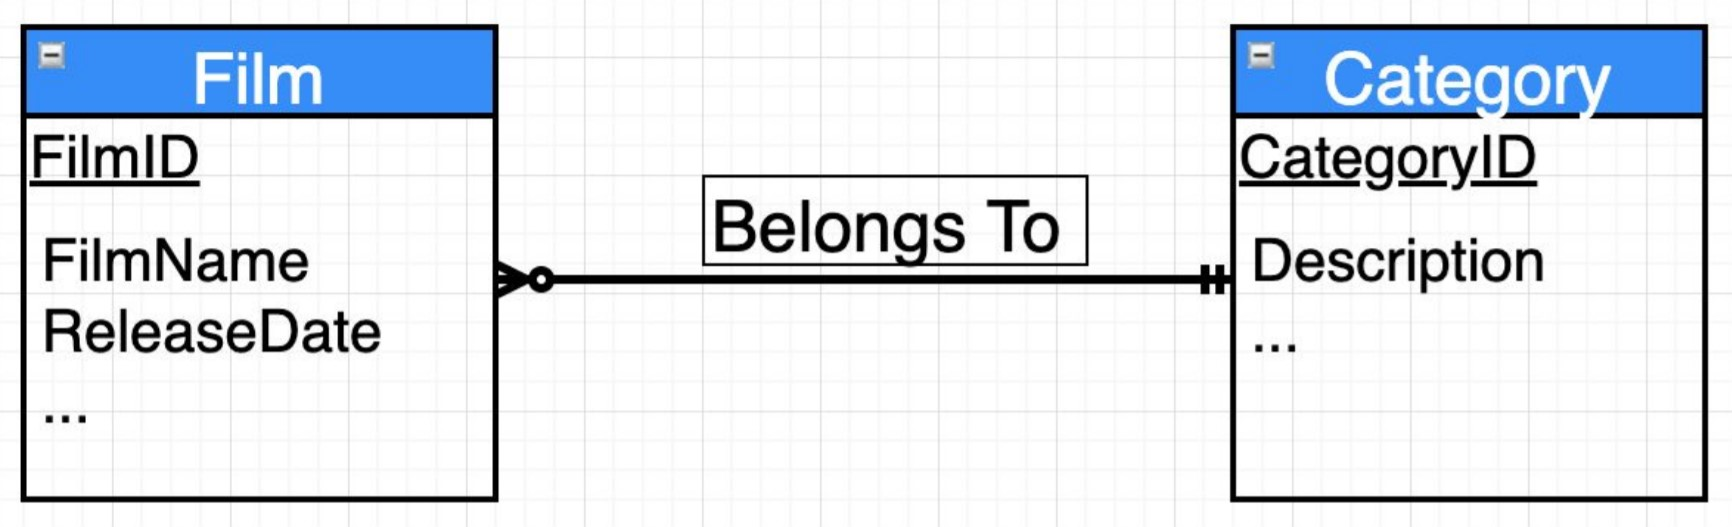
\includegraphics[width=0.75\textwidth]{unit-1/figures/er-diagram.jpg}
  \caption*{An entity relationship diagram.}
\end{figure}

The attributes of an entity are listed within its rectangle.
The primary key is underlined.

Relationships are named associations between entities.
Relationships provide associations in both directions.

\subsubsection{Cardinality}

\emph{Cardinality} provides a constraint on the number of instances of an entity that participate in a relationship.

\begin{figure}[htp]
  \centering
  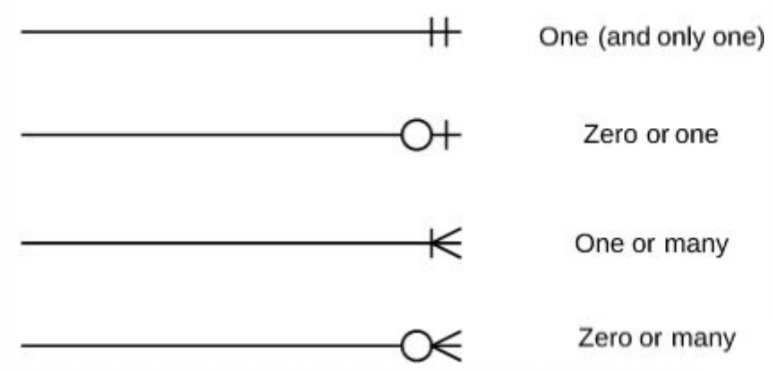
\includegraphics[width=0.6\textwidth]{unit-1/figures/cardinality-notation.jpg}
  \caption*{Cardinality notation.}
\end{figure}

\begin{table}[htp]
  \centering
  \caption*{Important cardinalities.}
  \begin{tabular}{ll}
    \toprule
    Name & Value \\
    \midrule
    Mandatory & Minimum cardinality \( \geq 1 \) \\ [1ex]
    Optional & Minimum cardinality \( = 0 \) \\ [1ex]
    Functional & Minimum cardinality \( = 1 \) \\ [1ex]
    \midrule
    One-to-one (1--1) & Maximum cardinality \( = 1 \) in both directions \\ [1ex]
    One-to-many (1--M) & Maximum cardinality \( = 1 \) in one direction \\
    & Maximum cardinality \( > 1 \) in the other direction \\ [1ex]
    Many-to-many (M--N) & Maximum cardinality \( > 1 \) in both directions \\
    \bottomrule
  \end{tabular}
\end{table}

\subsubsection{Foreign Keys and Weak Entities}

Relationships are translated to \emph{foreign~keys} in tables, except in the case of many-to-many relationships.

\emph{Weak~entities} are entities that do not have their own primary~key.
They must borrow attributes from other entities to form part or all of their primary~key.
Weak~entities are represented by rounded rectangles.
An underlined attribute of a weak~entity is not its primary key.
It is a key that is combined with the keys of one or more entities to provide a primary key.

\begin{figure}[htp]
  \centering
  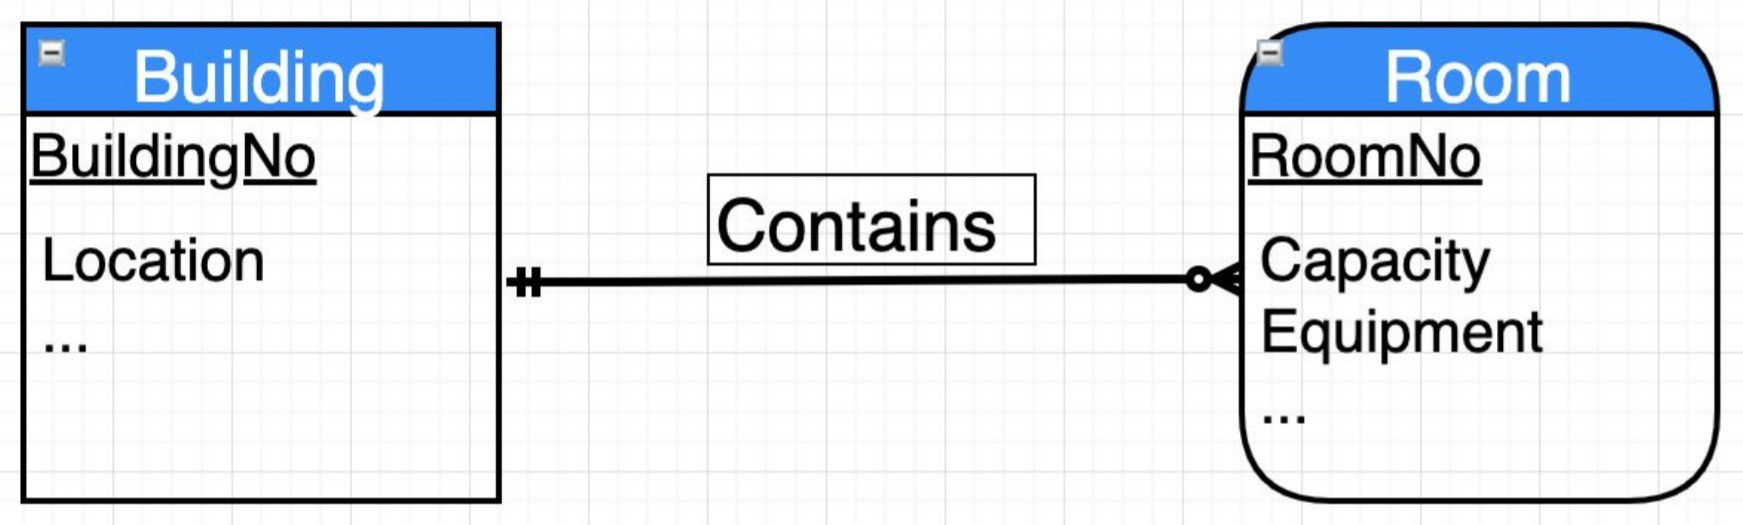
\includegraphics[width=0.75\textwidth]{unit-1/figures/weak-entity.jpg}
  \caption*{A weak entity relationship.}
\end{figure}

An \emph{identification relationship} provides one component of the primary key of a weak entity.
An \emph{identifying dependency} consists of one or more identification relationships that provide all of the primary key.
Sometimes an identification relationship and an identifying dependency are equivalent.

\subsubsection{Many-to-Many Relationships}

In a many-to-many relationship, the relationship itself can have attributes.
Theses attributes are listed below the relationship with an arrow pointing to them.

\begin{figure}[htp]
  \centering
  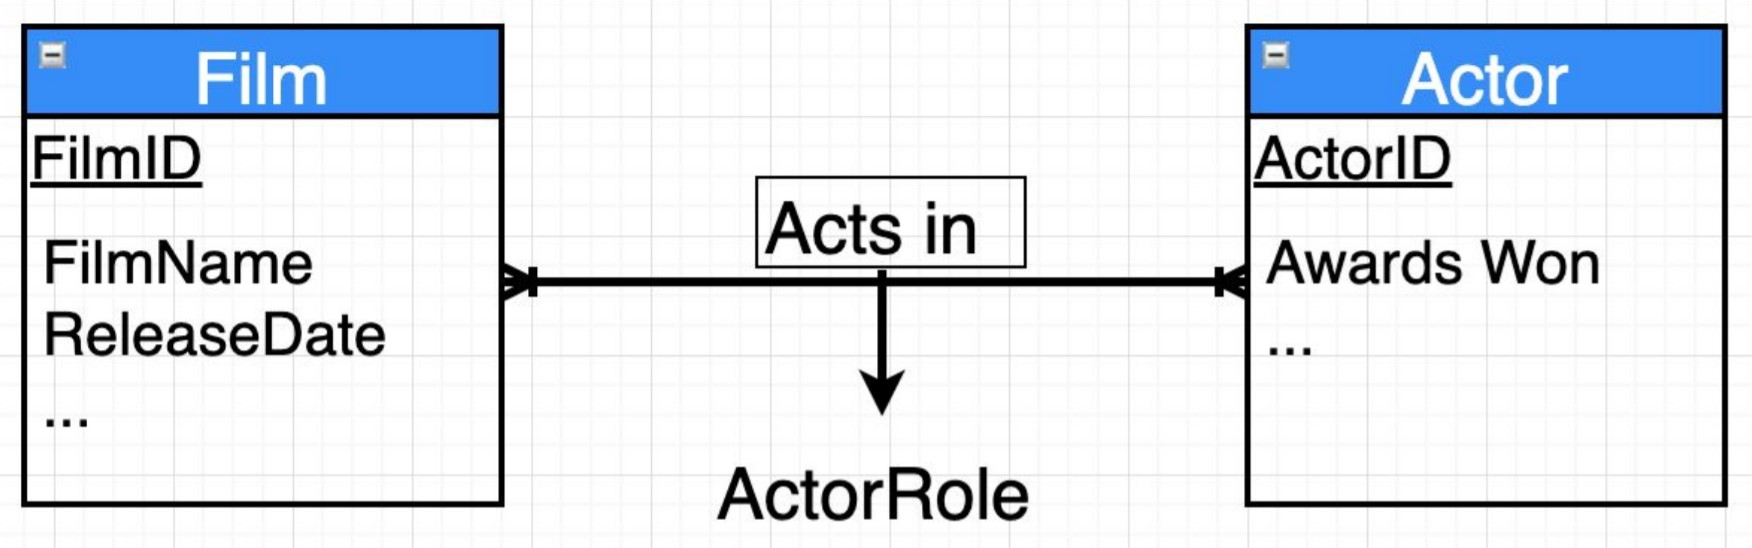
\includegraphics[width=0.75\textwidth]{unit-1/figures/relationship-attribute.jpg}
  \caption*{An attribute of a many-to-many relationship.}
\end{figure}

A many-to-many relationship can be replaced by an associate entity and two one-to-many relationships.

\begin{figure}[htp]
  \centering
  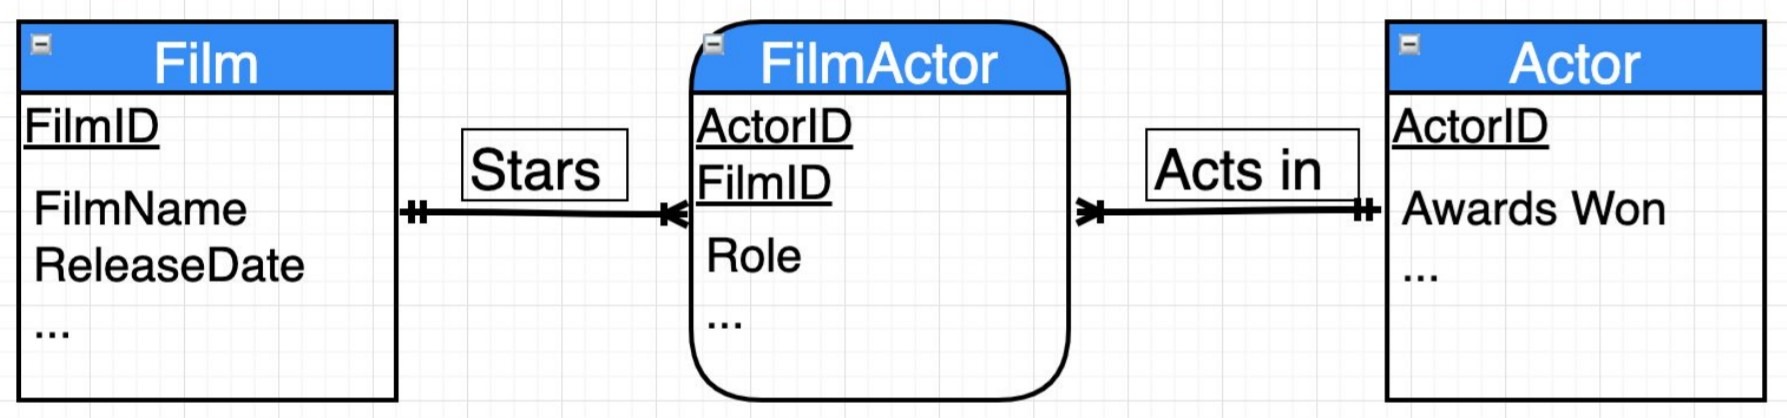
\includegraphics[width=\textwidth]{unit-1/figures/associate-entity.jpg}
  \caption*{An associate entity in a many-to-many relationship.}
\end{figure}

An associate entity provides additional information about the many-to-many relationship it implements.
By necessity, an associate entity is a weak entity that borrows the attributes of its primary~key from the entities between which it provides an association.

\subsubsection{\texorpdfstring{\( N \)}{N}-Way Relationships}

Sometimes --- though very rarely --- more than two entities are related to each other.
For example, a module may be taught by multiple lecturers, and a student is given a mark from each lecturer.
If it is only necessary to relate pairs of entities, such as which lecturers teach which modules, or which students are enrolled in which modules, an \( N \)-way relationship is not required.
If, however, it is necessary to store information associated with more than two entities, such as the mark given to a student from a lecturer for one section of a module, an \( N \)-way relationship is required.

\begin{figure}[htp]
  \centering
  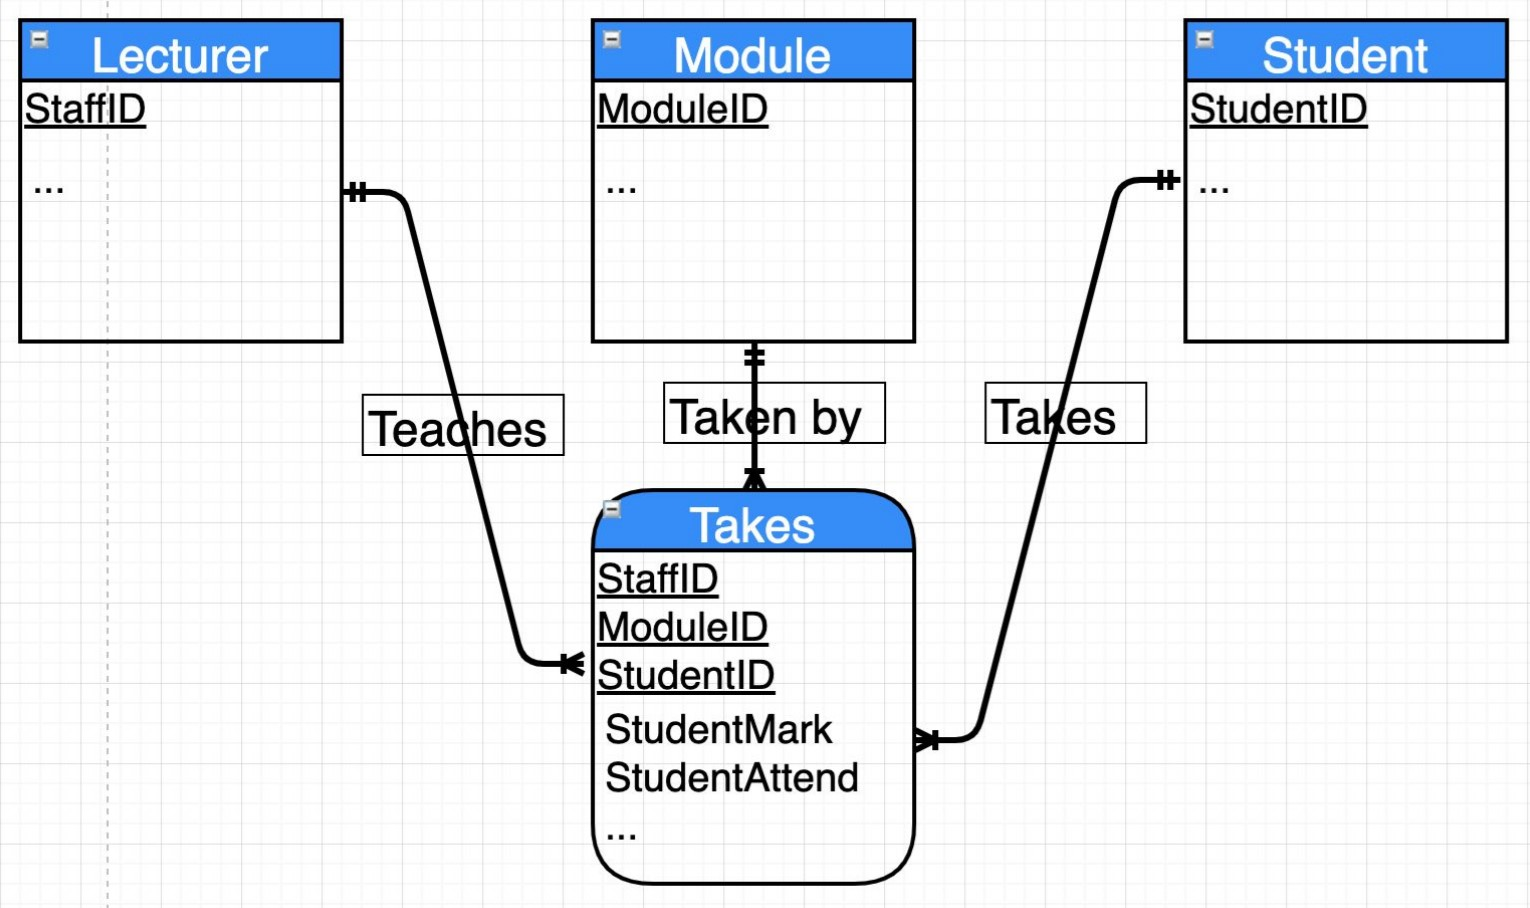
\includegraphics[width=\textwidth]{unit-1/figures/n-way-relationship.jpg}
  \caption*{An \( N \)-way relationship.}
\end{figure}

\subsubsection{Self-Identifying Relationships}

A \emph{self-identifying} (also \emph{self-referencing} or \emph{reflexive}) relationship is a relationship between an entity and itself.

\begin{figure}[htp]
  \centering
  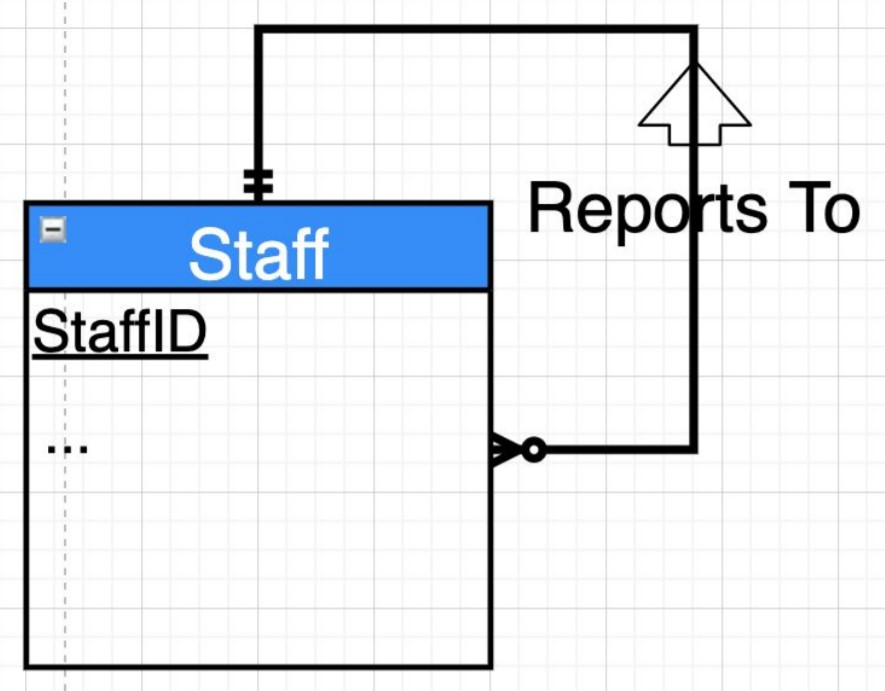
\includegraphics[width=0.4\textwidth]{unit-1/figures/self-identifying-relationship.jpg}
  \caption*{A self-identifying relationship.}
\end{figure}

All hierarchies are self-identifying relationships.
\begin{itemize}
  \item Biological classifications
  \item Organisational hierarchies
  \item Topic categories
\end{itemize}

In order to determine the cardinality of a self-identifying relationship, it is useful to draw an \emph{instance~diagram}.

\begin{figure}[htp]
  \centering
  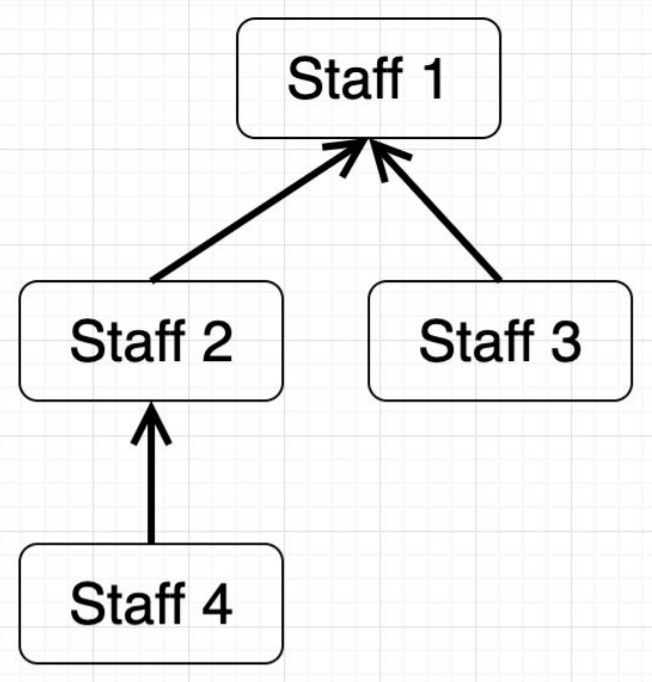
\includegraphics[width=0.3\textwidth]{unit-1/figures/instance-diagram.jpg}
  \caption*{An instance diagram of a self-identifying relationship.}
\end{figure}

A self-identifying relationship may require an associate entity, depending on its cardinality.
All self-identifying relationships can be translated to tables if many-to-many relationships are replaced by associate entities and one-to-many relationships.
